% Chapter 4

\chapter{Análisis} % Main chapter title


\label{Chapter4} % Change X to a consecutive number; for referencing this chapter elsewhere, use \ref{ChapterX}

En este capítulo se realiza el análisis de las diversas aplicaciones de dispositivos IoT y su implementación en redes de comunicaciones móviles 5G. Se comienza con una breve descripción de estas tecnologías, y después se profundiza en el caso de uso mMTC donde se mencionan los escenarios más comunes de implementación, su clasificación y sus características, además se revisa el estándar actual (NB-IoT\footnote{ Muchos\ de\ los\ modelos\ aqu\textrm{í}\ propuestos\ est\textrm{á}n\ basados\ en\ trabajos\ de\ la\ 3GPP,\ como\ se\ revis\textrm{ó}\ en\ el Capítulo \ref{Chapter2},\ la\ 3GPP,\ es\ una\ organizaci\textrm{ó}n\ que\ est\textrm{á}\ respaldada\ por\ organismos\ alrededor\ de\ todo\ el\ mundo,\ adem\textrm{á}s\ de\ que\ se\ trata\ del\ grupo\ que\ estandariza\ tecnolog\textrm{í}as\ como\ LTE-M\ y\ NB-IoT,\ de\ manera\ que\ es\ una\ indudable\ referencia\ en\ su\ ahora\ inmersi\textrm{ó}n\ en\ la\ estandarizaci\textrm{ó}n\ de\ 5G.}) que cumple con los requisitos para la implementación de mMTC. Finalmente también se revisan los KPIs propuestos para este tipo de escenarios.\newline

Por último, se detallan cuáles son los modelos y técnicas que se usan para caracterizar el modelo de despliegue, canal y de tráfico de dispositivos IoT en redes 5G y además se presenta la actual propuesta de técnica de acceso múltiple al medio no ortogonal (NOMA) y su enfoque hacia un entorno masivo de dispositivos (con el uso de \textit{clusterización}).


%----------------------------------------------------------------------------------------
%	SECTION 
%----------------------------------------------------------------------------------------

\section{RED 5G}

La NGMN define su visión de una red 5G de la siguiente manera: ``5G es un ecosistema de extremo a extremo para permitir una sociedad totalmente móvil y conectada."\newline

La anteriores generaciones de comunicaciones móviles (1G,{\dots},4G) han sido transformadoras en el sentido que fueron motivadas para mejorar los tradicionales KPIs de la red, sin embargo la nueva generación de comunicaciones móviles (5G) aparte de ser transformadora viene a ser disruptiva ante las generaciones anteriores ya que propone nuevas técnicas, modelos y KPIs que habilitarán una gama amplia de servicios con alta fiabilidad, ayudando a conformar toda una red heterogénea global móvil interconectada con altos índices de rendimiento.\newline

La investigación sobre los casos de uso de una red 5G y sus requisitos técnicos han sido realizadas por la ITU-R, el 3GPP y la NGMN:

\begin{figure}[th]
\centering
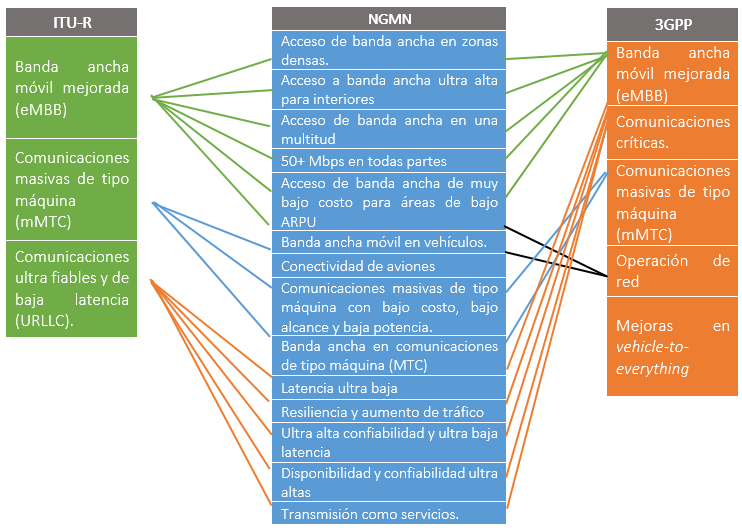
\includegraphics[scale=1]{Figures/Comparación de diversos escenarios de uso de la tecnología 5G}
\decoRule
\caption[Comparación de diversos escenarios de uso de la tecnología 5G por la UIT-R, el 3GPP y la NGMN]{Comparación de diversos escenarios de uso de la tecnología 5G por la UIT-R, el 3GPP y la NGMN}
\label{fig:5g}
\end{figure}

5G admitirá una gran variedad de casos de uso que están surgiendo ahora o surgirán en el futuro. Los diversos casos de uso tienen características y requisitos variables. Es útil agrupar innumerables casos de uso emergentes en varias familias de casos de uso. \newline

La \textit{Figura~\ref{fig:5g}} muestra las ocho familias de casos de uso por la NGMN con un ejemplo de caso de uso para cada familia, y sus correspondientes ejemplos de casos de uso con la 3GPP y la ITU-R.\newline

En términos generales, ITU-R ha concluido tres casos de uso para abordar la gran variedad de requisitos y características \parencite{5gMobileComms}:


\begin{enumerate}
    \item \textbf{Banda ancha móvil mejorada} \textbf{(eMBB)}: la banda ancha móvil aborda casos de uso centrados en el hombre para acceder a contenido multimedia, servicios y datos. La demanda de banda ancha móvil seguirá aumentando, lo que dará lugar a una banda ancha móvil mejorada. El escenario mejorado de uso de banda ancha móvil vendrá con nuevas áreas de aplicación y requisitos, además de las aplicaciones de banda ancha móvil existentes para un mejor rendimiento y una experiencia de usuario cada vez más perfecta.
    \item \textbf{Comunicaciones ultra fiables y de baja latencia (URLLC)}: este caso de uso tiene requisitos estrictos para capacidades tales como rendimiento, latencia y disponibilidad. Algunos ejemplos incluyen el control inalámbrico de la fabricación industrial o los procesos de producción, cirugía médica remota, automatización de la distribución en una red inteligente, seguridad en el transporte, manejo autónomo de automóviles, etc.
    \item \textbf{Comunicaciones masivas de tipo máquina (mMTC)}: este caso de uso se caracteriza por un gran número de dispositivos conectados que transmiten un volumen relativamente bajo de datos no sensibles al retardo. Los dispositivos deben ser de bajo costo y tener una batería de larga duración.
\end{enumerate}


%----------------------------------------------------------------------------------------
%	SECTION 
%----------------------------------------------------------------------------------------

\section{INTERNET DE LAS COSAS (IoT)}

El internet de las cosas (IoT) es una emergente y prometedora tecnología que habilitará la interconexión del mundo global a través de la conexión de objetos físicos (comúnmente dispositivos de bajo consumo) mediante el uso del internet \parencite{5GSurveyAkpaku}. Una de las características más importantes de esta tecnología es que ocupa la comunicación máquina a máquina (M2M) con el fin de que los dispositivos se conecten y comuniquen entre sí sin alguna intervención humana.\newline

Para habilitar esta tecnología se requiere el soporte para conexiones masivas, es decir, admitir la gran cantidad de sensores en una sola celda. Debido a que la mayoría de estos sensores deben operar durante varios años, la eficiencia energética en las transmisiones inalámbricas es un requisito importante. Además, se debe reducir el costo de implementación de tales sensores \parencite{IoT5GWire}.

%----------------------------------------------------------------------------------------
%	SECTION 
%----------------------------------------------------------------------------------------

\section{CLASIFICACIÓN Y ANÁLISIS DE LOS ÁMBITOS DE IoT}

La contribución en cuanto a la categorización de las aplicaciones de IoT que ya existen y las que se comenzarán a ver en años próximos, es vasta y no siempre compatible dependiendo del grupo que se consulte, de manera que se tomó como referencia el trabajo realizado en \parencite{NetTrafficIoT} como guía para los servicios que se espera brinden los nodos IoT en distintos ámbitos.\newline

La mayor parte de este trabajo está dedicada a la caracterización de las aplicaciones de IoT y sus dominios, los cuales se dividen en 8, específicamente: edificios inteligentes y vivienda (\textit{Smart buildings and living}), cuidado de la salud inteligente (\textit{Smart healthcare}), medio ambiente inteligente (\textit{Smart environment}), ciudades inteligentes (\textit{Smart city}), energía inteligente (\textit{Smart energy}), transporte y movilidad  inteligentes (\textit{Smart transport and mobility}), fabricación y venta inteligentes (\textit{Smart manufacturing and retail}), agricultura inteligente (\textit{Smart agriculture}). Para cada uno de los dominios se especifican aplicaciones típicas que se podrían encontrar, sus características de tráfico, las tecnologías de red más adecuadas para darles servicio entre otras cosas.\newline

La primera parte del análisis correspondió a la selección de los dominios que resultasen adecuados para el sistema que se diseña, es decir los dominios cuya red que les brindará servicio primordialmente será una red de área amplia de bajo consumo (LPWAN, \textit{Low Power Wide Area Network}). Esto se debe a que algunas de las aplicaciones en los dominios antes mencionados están pensadas para redes de distintas características en las que tecnologías como RFID, \textit{Bluetooth }o \textit{ZigBee }podrían ser una mejor solución. A continuación se presenta la caracterización de cada uno de los dominios que en \parencite{NetTrafficIoT} se consideran viables para redes LPWAN.\newline

\subsection{Ciudades inteligentes \textit{(Smart City)}:}

Con el rápido incremento de la población y su concentración en poblaciones urbanas, se ha convertido en una prioridad la reducción del uso de recursos públicos, así como la reducción de costos de operación del día a día de una ciudad, ambas de la manera más óptima posible. Las aplicaciones en este dominio tratan justamente de abordar estos problemas y los servicios que brindan son bastante variados, los ejemplos van desde el control de luminarias hasta el manejo de desechos, estos y otros  pueden encontrarse en la \textit{Tabla~\ref{tab:smartcity}}, acompañados de más información tal como la caracterización de su tráfico y su demanda de QoS.\newline

\begin{table}
\caption{Características de las aplicaciones de Ciudades Inteligentes}
\label{tab:smartcity}
%\centering
\begin{tabular}{*{5}{m{3cm}}}\\
\textbf{\textit{Servicio}} & \textbf{\textit{Tamaño de red}} & \textbf{\textit{Tasa de tráfico}} & \textbf{\textit{Demanda de QoS}} & \textbf{\textit{Fuente de energía}} \\ \hline
\textit{Monitoreo del consumo de agua y electricidad en la ciudad} & \footnotesize{Media a grande, cientos a miles de dispositivos} & \footnotesize{Periódico, 1 msj cada 10 min por dispositivo} & \footnotesize{Baja, tolerante al retardo 1 min} & \footnotesize{Alimentado por la red eléctrica/ autoalimentado} \\ 
\textit{Control de iluminación} & \footnotesize{Grande, miles de dispositivos} & \footnotesize{Aleatorio, poco frecuente} & \footnotesize{Media, tolerante al retardo 15 seg} & \footnotesize{Alimentado por la red eléctrica }\\ 
\textit{Vigilancia de estacionamientos} & \footnotesize{Grande, miles de dispositivos} & \footnotesize{Aleatorio, poco frecuente} & \footnotesize{Media, tolerante al retardo 10 seg} & \footnotesize{Alimentado por batería }\\ 
\textit{Control del tráfico} & \footnotesize{Grande, miles de dispositivos} & \footnotesize{Periódico, 1 msj cada 10 min por dispositivo, aleatorio para alarmas} & \footnotesize{Media, tolerante al retardo 15 seg, alta para alarmas} & \footnotesize{Alimentado por batería} \\ 
\textit{Mantenimiento de deshechos} & \footnotesize{Grande, miles de dispositivos} & \footnotesize{Aleatorio, poco frecuente} & \footnotesize{Media, tolerante al retardo 30 seg} & \footnotesize{Alimentado por batería }\\ 
\textit{Monitoreo de condiciones urbanas} & \footnotesize{Media a grande, cientos a miles de dispositivos} & \footnotesize{Periódico, 1 msj cada 15 min por dispositivo, aleatorio para alarmas} & \footnotesize{Media, tolerante al retardo 30 seg, alta para alarmas} & \footnotesize{Alimentado por batería }\\ 
\textit{Monitoreo de la salud estructural de edificios} & \footnotesize{Media a grande, cientos a miles de dispositivos} & \footnotesize{Periódico, 1 msj cada 15 min por dispositivo, aleatorio para alarmas} & \footnotesize{Media, tolerante al retardo 30 seg, alta para alarmas} & \footnotesize{Alimentado por batería} \\ 
\end{tabular}
\end{table}

\subsection{Ambiente inteligente \textit{(Smart Environment)}}
\subsection{Energía inteligente \textit{(Smart Energy)}:}
\subsection{Transporte y movilidad inteligentes \textit{(Smart Transport and Mobility)}:}

%----------------------------------------------------------------------------------------
%	SECTION 
%----------------------------------------------------------------------------------------

\section{CARACTERÍSTICAS DEL ESCENARIO A IMPLEMENTAR}
\subsection{Análisis de las aplicaciones de IoT y selección de casos considerados}
\subsection{Análisis de las tecnologías para IoT y selección de casos considerados}
\subsection{Análisis del estándar NB-IoT}

%----------------------------------------------------------------------------------------
%	SECTION 
%----------------------------------------------------------------------------------------

\section{INDICADORES CLAVE DE RENDIMIENTO (KPIs)}

%----------------------------------------------------------------------------------------
%	SECTION 
%----------------------------------------------------------------------------------------

\section{ANÁLISIS DE MODELOS PARA LA EVALUACIÓN DE REDES 5G/IoT}
\subsection{MODELO DE DESPLIEGUE DE BSs Y UEs}
\subsection{MODELO DE CANAL}
\subsection{ESQUEMA DE ACCESO MÚLTIPLE AL MEDIO}
\subsection{MODELOS DE TRÁFICO}


\myworries{TODO: Faltan palabras en ingles en italicas en este capitulo}